\chapter{Inference on Czech News sample}\label{inference}

\begin{itemize}
    \item abstract,headline, text bias correlation
    \item vbias progress over time for one domain
    \item plot the difference between domains
    \item plot the difference between topics
    \item info about 'commentary' articles is presented! super
    \item length correlates with bias -> perhaps longer text leaves more space for bias
    \item quoting has no correlation with bias
    \item čím víc článků je, tím menší je bias.. :(
\end{itemize}

vhodný články
\begin{enumerate}
    \item \url{https://www.novinky.cz/domaci/clanek/jak-cist-volby-294694}
    \item tahle je asi nej ta pod timhle
    \item \url{https://www.novinky.cz/zahranicni/evropa/150611-v-rakouskych-volbach-podle-pruzkumu-triumfuji-pravicovi-populiste.html}
\end{enumerate}

An example of classified news article can be seen in figure \ref{fig:demoarticle}.

\begin{figure}
\makebox[\textwidth][c]{
  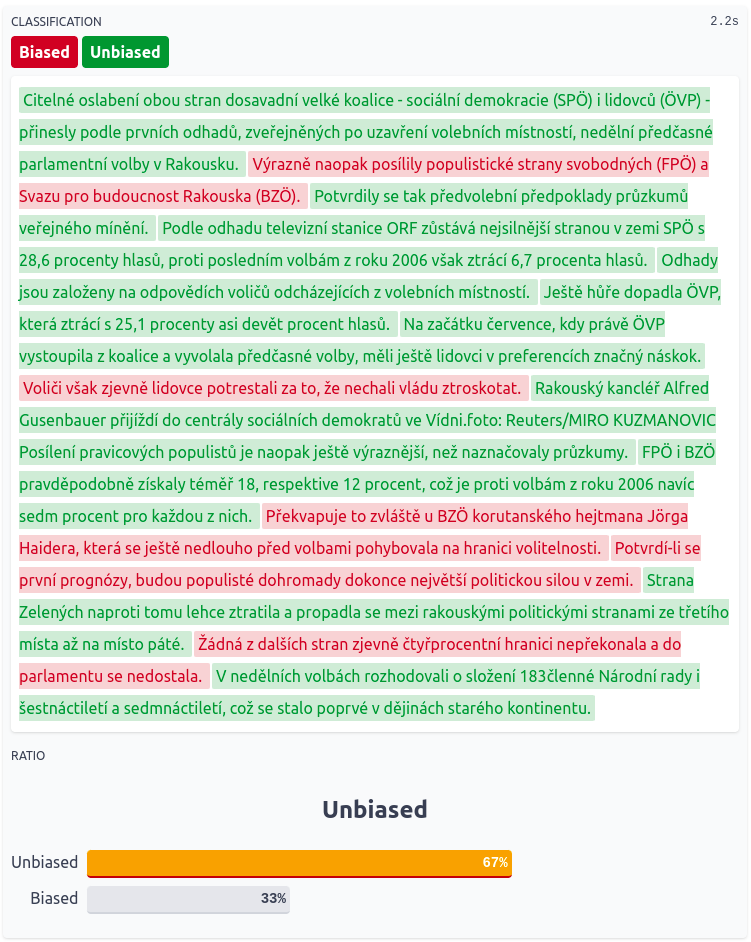
\includegraphics[scale=0.5]{my_modules/multimedia/article_example.png}
  \caption{Example of classified article.}
  \label{fig:demoarticle}
  }
\end{figure}

\subsection{Demo}
Additionally, I provide a simple web demo for the reader to experiment with\footnote{\url{https://huggingface.co/spaces/horychtom/czech_media_bias_detection}}. The use of the demo can be seen in \ref{fig:demodemo}. The backend runs on HuggingFace's spaces\footnote{\url{https://huggingface.co/spaces}} which is a free hosting service for demonstration of \gls{ml} applications. 

The user can insert arbitrary text in Czech language; text is then split into sentences and classified individually. Then the average percentage bias score of the text is displayed. An \textit{interpret} button allows the user to further inspect the classification.

\begin{figure}
\makebox[\textwidth][c]{
  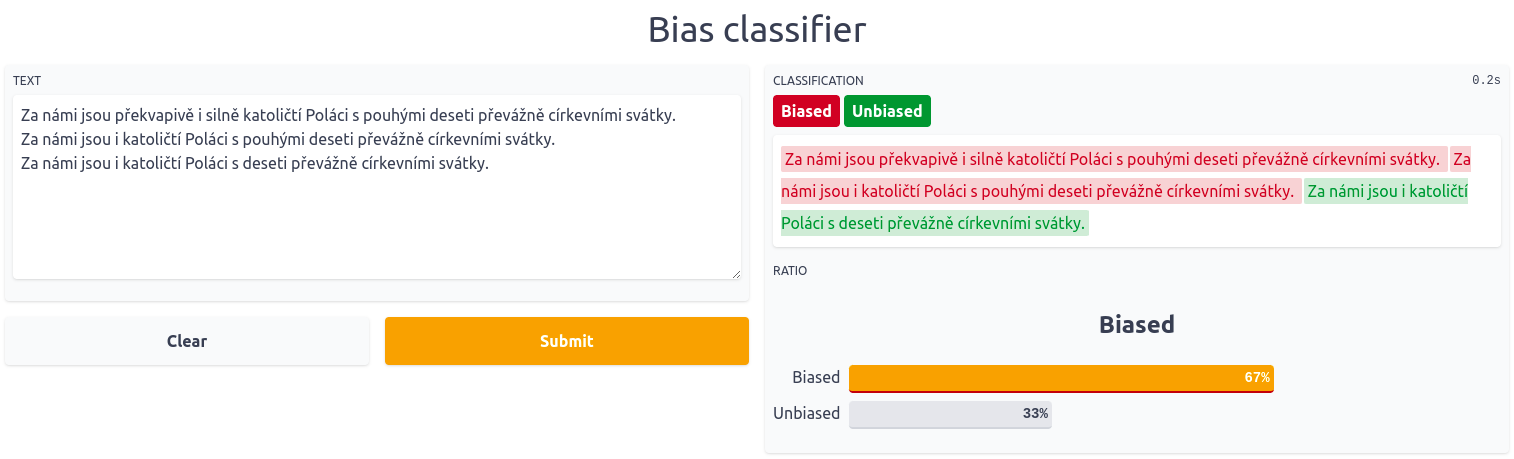
\includegraphics[scale=0.3]{my_modules/multimedia/bias.png}
  \caption{Example of the bias classifier demo usage. Red and blue color represent the biased and unbiased annotation respectively.}
  \label{fig:demodemo}
  }
\end{figure}
